\documentclass[a4paper,11pt]{article}

\usepackage[utf8]{inputenc}

\usepackage{graphicx}
\usepackage{caption}
\usepackage{subcaption}

\usepackage{pgfplots}
\pgfplotsset{compat=1.18} 

\usepackage{minted}
\usepackage{siunitx}
\usepackage{tikz}
\usetikzlibrary{positioning}

\begin{document}

\title{
    \textbf{Breadth-first search}
}
\author{Mo Wang}
\date{Spring 2026}

\maketitle

\section*{Introduction}

This report presents an implementation of breadth-first traversal (BFS) for binary trees. Unlike depth-first traversal that explores one sub-branch completely before moving to another, breadth-first traversal visits all nodes at the current depth before proceeding to the next. This approach is useful when the search element is expected near the root, since BFS guarantees that all nodes at shallower depths are examined before nodes at deeper levels.

\section*{Breadth-first traversal}

A breadth-first traversal may seem straightforward when looking at a complete binary tree being drawn on paper. Since each level is visually aligned, nodes belonging to the same depth can easily be seen and traced. However, implementing an algorithm for BFS can be tricky, since the algorithm does not inherently carry information of all nodes at an exact depth. Although finding the left and right children is trivial, since the binary tree node  carries respective pointer addresses, wrapping around from the rightmost node of one depth being traversed to the leftmost node of the depth below becomes difficult.

\subsection*{Queue-based solution}
The solution relies on maintaining an explicit queue of nodes later to be visited. It mainly acts as a space for missing structural information that the tree itself does not provide.

In breadth-first traversal, we repeatedly \emph{dequeue} the first node from the queue, \emph{print} (visit) it, and then \emph{enqueue} its children (left child first, then right child) if they exist. Because the left child is enqueued before the right child, the leftmost child is dequeued first, ensuring that all nodes at a given depth are processed before any node at the next depth. This process repeats until the queue is empty. Initially, if the root exists, it is enqueued once. The algorithm becomes especially clear on a concrete alphabetic tree, as shown in Figure~\ref{fig:bfs-traversal}.

\noindent Breadth-first traversal proceeds in every step as follows:

(1) if the queue is empty, stop; otherwise

(2) \emph{dequeue} the first node and \emph{print} it;

(3) \emph{enqueue} its left child (if any), then its right child (if any);

(4) repeat from (1).


\begin{figure}[htbp]
\centering

% ====== GLOBAL STYLES ======
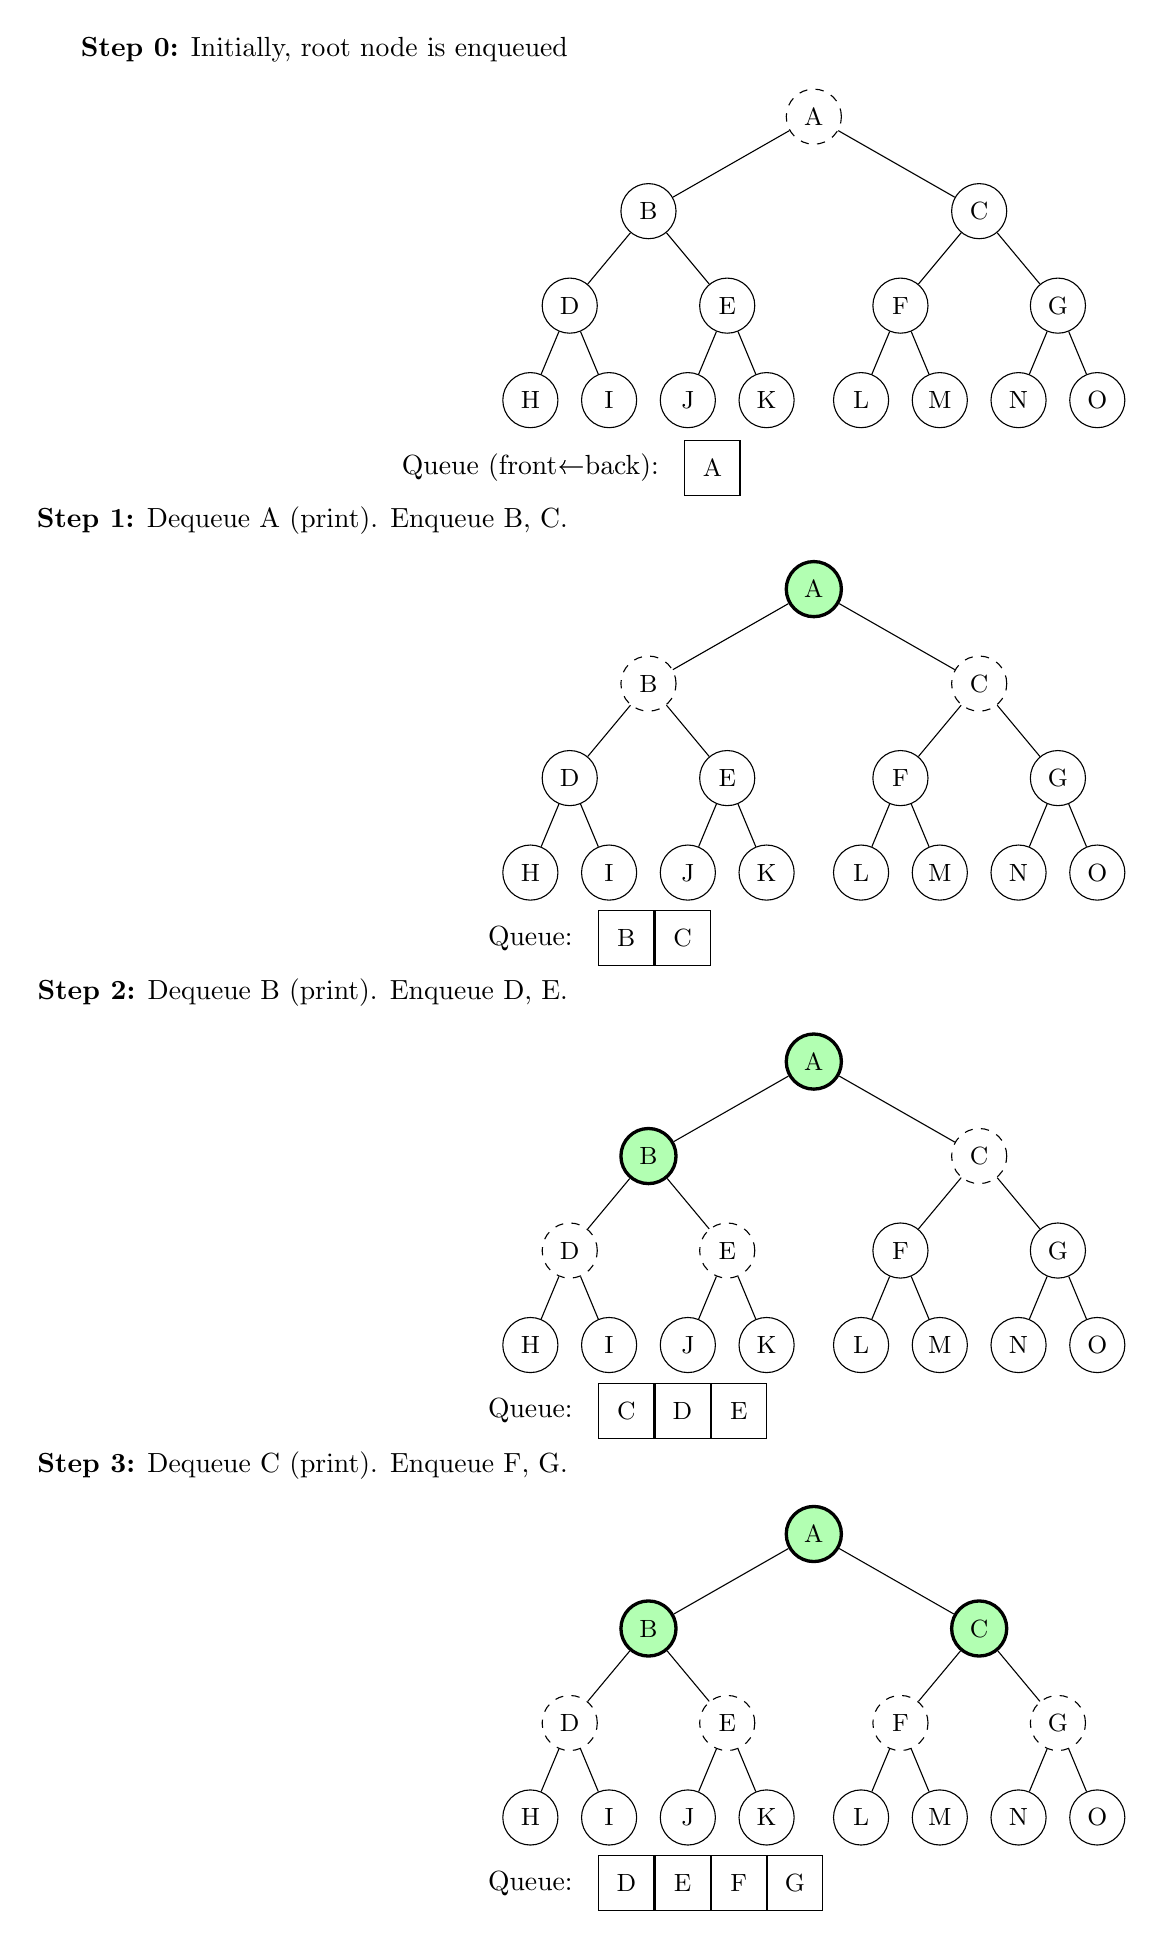
\begin{tikzpicture}[
  level distance=12mm,
  sibling distance=30mm,
  level 1/.style={sibling distance=42mm},
  level 2/.style={sibling distance=20mm},
  level 3/.style={sibling distance=10mm},
  node/.style={circle, draw, minimum size=7mm, font=\small},
  printed/.style={node, fill=green!30, very thick},
  current/.style={node, fill=orange!35, very thick},
  queued/.style={node, dashed},
  box/.style={draw, minimum width=7mm, minimum height=7mm, font=\small}
]

% ======================================================
% =============== STEP 0 ===============================
% ======================================================
\begin{scope}[yshift=8cm]
\node (A0) [queued] {A}
  child { node (B0) [node] {B}
    child { node (D0) [node] {D}
      child { node (H0) [node] {H} }
      child { node (I0) [node] {I} }
    }
    child { node (E0) [node] {E}
      child { node (J0) [node] {J} }
      child { node (K0) [node] {K} }
    }
  }
  child { node (C0) [node] {C}
    child { node (F0) [node] {F}
      child { node (L0) [node] {L} }
      child { node (M0) [node] {M} }
    }
    child { node (G0) [node] {G}
      child { node (N0) [node] {N} }
      child { node (O0) [node] {O} }
    }
  };

\node[above=5mm of A0, anchor=east, xshift=-30mm] {\textbf{Step 0:} Initially, root node is enqueued};

% queue
\node[below=2mm of H0] (q0label) {Queue (front←back):};
\node[box, right=2mm of q0label] (q0a) {A};
\end{scope}

% ======================================================
% =============== STEP 1 ===============================
% ======================================================
\begin{scope}[yshift=2cm]
\node (A1) [printed] {A}
  child { node (B1) [queued] {B}
    child { node (D1) [node] {D}
      child { node (H1) [node] {H} }
      child { node (I1) [node] {I} }
    }
    child { node (E1) [node] {E}
      child { node (J1) [node] {J} }
      child { node (K1) [node] {K} }
    }
  }
  child { node (C1) [queued] {C}
    child { node (F1) [node] {F}
      child { node (L1) [node] {L} }
      child { node (M1) [node] {M} }
    }
    child { node (G1) [node] {G}
      child { node (N1) [node] {N} }
      child { node (O1) [node] {O} }
    }
  };

\node[above=5mm of A1, anchor=east, xshift=-30mm] {\textbf{Step 1:} Dequeue A (print). Enqueue B, C.};

% queue
\node[below=2mm of H1] (q1label) {Queue:};
\node[box, right=2mm of q1label] (q1b) {B};
\node[box, right=0mm of q1b] (q1c) {C};
\end{scope}

% ======================================================
% =============== STEP 2 ===============================
% ======================================================
\begin{scope}[yshift=-4cm]
\node (A2) [printed] {A}
  child { node (B2) [printed] {B}
    child { node (D2) [queued] {D}
      child { node (H2) [node] {H} }
      child { node (I2) [node] {I} }
    }
    child { node (E2) [queued] {E}
      child { node (J2) [node] {J} }
      child { node (K2) [node] {K} }
    }
  }
  child { node (C2) [queued] {C}
    child { node (F2) [node] {F}
      child { node (L2) [node] {L} }
      child { node (M2) [node] {M} }
    }
    child { node (G2) [node] {G}
      child { node (N2) [node] {N} }
      child { node (O2) [node] {O} }
    }
  };

\node[above=5mm of A2, anchor=east, xshift=-30mm] {\textbf{Step 2:} Dequeue B (print). Enqueue D, E.};

% queue
\node[below=2mm of H2] (q2label) {Queue:};
\node[box, right=2mm of q2label] (q2c) {C};
\node[box, right=0mm of q2c] (q2d) {D};
\node[box, right=0mm of q2d] (q2e) {E};
\end{scope}

% ======================================================
% =============== STEP 3 ===============================
% ======================================================
\begin{scope}[yshift=-10cm]
\node (A3) [printed] {A}
  child { node (B3) [printed] {B}
    child { node (D3) [queued] {D}
      child { node (H3) [node] {H} }
      child { node (I3) [node] {I} }
    }
    child { node (E3) [queued] {E}
      child { node (J3) [node] {J} }
      child { node (K3) [node] {K} }
    }
  }
  child { node (C3) [printed] {C}
    child { node (F3) [queued] {F}
      child { node (L3) [node] {L} }
      child { node (M3) [node] {M} }
    }
    child { node (G3) [queued] {G}
      child { node (N3) [node] {N} }
      child { node (O3) [node] {O} }
    }
  };

\node[above=5mm of A3, anchor=east, xshift=-30mm] {\textbf{Step 3:} Dequeue C (print). Enqueue F, G.};

% queue
\node[below=2mm of H3] (q3label) {Queue:};
\node[box, right=2mm of q3label] (q3d) {D};
\node[box, right=0mm of q3d] (q3e) {E};
\node[box, right=0mm of q3e] (q3f) {F};
\node[box, right=0mm of q3f] (q3g) {G};
\end{scope}

\end{tikzpicture}

\caption{Breadth-first search (BFS) on a complete binary tree}
\label{fig:bfs-traversal}
\end{figure}

\subsection*{Cases with different sized trees}

To verify the breadth-first traversal and the queue usage, several tree shapes and sizes are tested, and both the printed order and (briefly) the queue’s front$\leftarrow$back evolution are observed. These experiments complement the assignment’s request to try different sized trees and ensure to understand how the queue is used.

\paragraph{1) Single-node tree.}

\emph{Structure:} only the root (1 root node A).

\emph{Queue:} Enqueue \texttt{A} $\rightarrow$ Dequeue \texttt{A} $\rightarrow$ empty.

\begin{minted}{text}
Input tree:    A
BFS output:    A
\end{minted}

\paragraph{2) Right-skewed chain (3 nodes).}

\emph{Structure:} A→B→C, where each node has only a right child.

\emph{Queue (sketch):} Enqueue \texttt{A}; pop \texttt{A}, enqueue \texttt{B}; pop \texttt{B}, enqueue \texttt{C}; pop \texttt{C}, then empty.

\begin{minted}{text}
Input tree (shape):    A
                        \
                         B
                          \
                           C
BFS output:            A B C
\end{minted}

\paragraph{3) Incomplete tree (root with two children; left child has only a left).}

\emph{Structure:} Root \texttt{A}; children \texttt{B} and \texttt{C}; node \texttt{B} has left child \texttt{D}; nodes \texttt{C} and \texttt{D} are leaves.

\emph{Queue (sketch):} Start \texttt{[A]}; pop \texttt{A}, enqueue \texttt{B,C} $\Rightarrow$ \texttt{[B,C]}; pop \texttt{B}, enqueue \texttt{D} $\Rightarrow$ \texttt{[C,D]}; pop \texttt{C} $\Rightarrow$ \texttt{[D]}; pop \texttt{D} $\Rightarrow$ empty.

\begin{minted}{text}
Input tree (shape):    A
                      / \
                     B   C
                    /
                   D
BFS output:        A B C D
\end{minted}

\paragraph{4) Complete four-level alphabetic tree (A–O).}
This is the same tree used in Figure~\ref{fig:bfs-traversal}, which demonstrates the queue contents and step labels. 
\emph{Expected BFS:} \texttt{A B C D E F G H I J K L M N O}. 
This confirms that enqueuing the left child before the right child yields left-to-right processing within each depth, and that all nodes at depth $d$ are visited before any node at depth $d{+}1$.

\medskip


\subsection*{Queue}

Implementing the algorithm requires another queue data-structure, which has already been implemented in previous assignment. An array-based queue is used to reduce fragmentation and faster access compared to linked-list based queue, although it causes latency spikes during resizes. The code is similar to the array-queue implementation, but hold pointer addresses to tree nodes \texttt{node *} instead of integers \texttt{int}.

\begin{minted}{c}
typedef struct arrayqueue{
    node **array;        // Array of node pointers
    unsigned int capacity; // Total capacity of the array
    unsigned int first;    // Index of front element
    unsigned int last;     // Index for next insertion
} arrayqueue;
\end{minted}

The provided functions for queue operations are:

\begin{itemize}
    \item \texttt{arrayqueue *arrayqueue\_create()}  
          -- Allocates and initializes an empty queue.

    \item \texttt{void arrayqueue\_free(arrayqueue *aq)}  
          -- Deallocates all internal memory associated with the queue.

    \item \texttt{bool arrayqueue\_empty(arrayqueue *aq)}  
          -- Returns \texttt{true} if the queue contains no elements.

    \item \texttt{void arrayqueue\_enqueue(arrayqueue* aq, node *v)}  
          -- Enqueues a node pointer to the the queue.

    \item \texttt{node *arrayqueue\_dequeue(arrayqueue *aq)}  
          -- Dequeues and returns the node pointer from the queue.
\end{itemize}

\subsection*{Implementation}

The code mechanism is simple as following: Initially, the root node is automatically enqueued into the queue. As the queue is not empty, the element is dequeued, traversed and its children enqueued into the queue, where the process repeats over.

To prevent the pathological case of empty tree, the root node is checked to be existent before pushing it into the queue.

\begin{minted}{c}
void breadth_first_print(const tree *tr){
    if (!tr || !tr->root) return; // Invalid tree
    
    // Create queue for BFS traversal
    arrayqueue *queue = arrayqueue_create();
    arrayqueue_enqueue(queue, tr->root);
    
    // Process nodes level by level
    while (!arrayqueue_empty(queue)) {
        node *current = arrayqueue_dequeue(queue);
        
        // Visit current node
        printf("%d ", current->value);
        
        // Enqueue children for later processing (left to right)
        if (current->left != NULL) 
            arrayqueue_enqueue(queue, current->left);
        if (current->right != NULL) 
            arrayqueue_enqueue(queue, current->right);
    }
    
    // Clean up
    arrayqueue_free(queue);
    printf("\n");
}
\end{minted}

In a properly constructed binary tree, infinite branches are impossible, which means the algorithm will sooner or later be terminated. This is because trees are finite acyclic structures with its nodes carrying children pointer addresses to nodes that does not belong to the previous ones. However, if the structure contains cycles due to invariant violations, the traversal could become non-terminating.

\section*{Lazy breadth-first implementation}

\subsection*{Create sequence}

In some cases, a tree can be traversed partially by lazy loading. In this case, a new data structure, named \texttt{sequence}, is constructed for holding a traversal queue, which is essential for containing traversal data. This is similar to initializing procedures in BFS traversal before entering the while loop.

\begin{minted}{c}
sequence *create_sequence(tree *tr){
    // Validate input: tree must exist and have a root
    if (tr == NULL || tr->root == NULL) return NULL;
    
    // Allocate memory for the sequence structure
    sequence *seq = (sequence *) malloc(sizeof(sequence));
    if (seq == NULL) return NULL; // malloc failed
    
    // Create the internal queue for BFS traversal
    seq->queue = arrayqueue_create();
    if (seq->queue == NULL) {
        free(seq); // Queue creation failed, clean up sequence
        return NULL;
    }
    // Initialize queue with root node to start traversal
    arrayqueue_enqueue(seq->queue, tr->root);
    return seq;
}
\end{minted}

\subsection*{Free sequence}

Since the data structure is allocated using \texttt{malloc}, a procedure for de-allocation is also required.

\begin{minted}{c}
void free_sequence(sequence *seq){
    if (seq == NULL) return; // Validate sequence pointer
    arrayqueue_free(seq->queue); // Free the internal queue
    free(seq); // Free the sequence structure itself
}
\end{minted}

\subsection*{Next}

Traversing the tree can be accomplished by requesting each element using the traversal structure \texttt{sequence} with the function \texttt{int next(sequence* seq)}. It essentially contains the logic inside the while loop of the BFS traversal algorithm. When the end of the tree is reached, the function returns 0 as a placeholder value.

\begin{minted}{c}
int next(sequence *seq){
    // Validate sequence pointer
    if (seq == NULL) return 0;
    
    // Check if there are more nodes to process
    if (arrayqueue_empty(seq->queue)){
        return 0; // Traversal complete
    }
    
    // Get the next node from the queue
    node *nd = arrayqueue_dequeue(seq->queue);
    if (nd == NULL){
        return 0; // Dequeue failed (shouldn't happen if queue not empty)
    }
    
    // Enqueue left child if it exists
    if (nd->left != NULL) arrayqueue_enqueue(seq->queue, nd->left);
    // Enqueue right child if it exists
    if (nd->right != NULL) arrayqueue_enqueue(seq->queue, nd->right);
    
    // Return the value of the current node
    return nd->value;
}
\end{minted}

\subsection*{Lazy BFS}

Using this structure, a tree can be constructed where its first three values can be extracted and another two later.

\begin{minted}{c}
  tree *myTree = construct_tree();
  // construct the tree
  
  sequence *seq = create_sequence(myTree);
  printf("%d ", next(seq));
  printf("%d ", next(seq));
  printf("%d ", next(seq));

  // other tasks

  printf("%d ", next(seq));
  printf("%d ", next(seq));

  // Cleanup
  free_sequence(seq);
  free_tree(myTree);
\end{minted}

Since the sequence stores a queue of node pointer addresses that are yet to be visited, calling next(seq) again after modifying the tree may yield incorrect traversal for the following nodes, since the queue contains stale data after modification.

\subsection*{Mutation Hazards: Queue Staleness and Undefined Behavior in Lazy BFS}

For node insertions, incorrect traversal order will occur if leaf node pointer addresses are already pushed in the queue. 
Otherwise, traversal will not be affected, considering that a node is usually attached as the leaf node, which is not loaded into the queue yet.

On the other hand, node deletions during tree traversal can cause incorrect traversal behavior and potentially undefined behavior. If the queue contains a pointer to the node being deleted, as the traversal function \texttt{next(seq)} tries to process it, it may de-reference a freed pointer, which can cause either a crash, an undefined behavior, or traversal of arbitrary garbage memory being misinterpreted as a node structure.

In either of the cases, A BFS lazy sequence becomes meaningless when the tree is mutated. So, a BFS "lazy sequence" is therefore not stable under mutation of an underlying tree. To avoid these issues, the tree should either be treated as immutable during traversal or the traversal structure should be reset whenever the tree is modified.

\section*{Conclusion}

In summary, breadth-first traversal provides a clear and systematic method for visiting all nodes in a binary tree level by level. By maintaining an explicit queue of nodes yet to be processed, the traversal guarantees that all nodes at a given depth are visited before any nodes at the next depth. This level-order behavior makes BFS particularly useful when elements are expected to appear near the root or when processing naturally occurs in depth-wise layers.

The lazy breadth-first approach further extends this idea by encapsulating the traversal state inside a separate \texttt{sequence} structure, allowing nodes to be retrieved incrementally through the \texttt{next(seq)} function. This enables partial traversal, pausing, and later resuming without restarting from the root.

However, the correctness of such a lazy sequence depends on the tree remaining unchanged during traversal. Any mutation of the underlying tree can invalidate the stored queue: insertions may disrupt the intended visitation order, while deletions may leave stale or dangling pointers that can lead to incorrect behavior or undefined memory access. Consequently, a BFS lazy sequence is only meaningful when the tree is treated as immutable for the duration of the traversal, or when the traversal structure is reset after any modification.

Overall, breadth-first traversal remains a reliable method for depth-wise exploration of tree structures, and the lazy variant offers additional flexibility as long as the underlying tree is not altered mid-traversal.

\end{document}